\documentclass[conference]{IEEEtran}
\usepackage{times}

% numbers option provides compact numerical references in the text. 
\usepackage[numbers]{natbib}
\usepackage{multicol}
\usepackage[bookmarks=true]{hyperref}

% newly defined commands
%%%%%%%%%%%%%%%%%%%%%%%%%%%%%%%%%%%%%%%%%%%%%%%%%%%%%%%%
\usepackage{amsmath} % assumes amsmath package installed
\usepackage{amssymb}  % assumes amsmath package installed
\usepackage{bm}
\usepackage{xcolor}
\usepackage{graphicx}
\usepackage{cleveref}
\usepackage{multirow}
\usepackage{makecell}
\usepackage{booktabs}
\usepackage{todonotes}
\usepackage{chngcntr}
\usepackage{dsfont}
% \usepackage[toc,page]{appendix}
\crefalias{section}{appendix}

%%% Theorem, defintions
\usepackage{amsthm}
\newtheorem{definition}{Definition}
\newcommand{\parents}{\mathrm{Pa}} 

%%%
%Shortcuts
\usepackage{xspace}
% Add a period to the end of an abbreviation unless there's one
% already, then \xspace.
\makeatletter
\DeclareRobustCommand\onedot{\futurelet\@let@token\@onedot}
\def\@onedot{\ifx\@let@token.\else.\null\fi\xspace}
\makeatother

\newcommand{\eg}{e.g\onedot}
\newcommand{\ie}{i.e\onedot}
\newcommand{\cf}{cf\onedot}
\newcommand{\etc}{etc\onedot}
\newcommand{\wrt}{w.r.t\onedot}
\newcommand{\indep}{\perp \!\!\! \perp}
%%%

% Naming our method
\newcommand{\algo}[1]{\textsc{#1}}
\newcommand{\method}{\algo{CAIMAN}\xspace}
\def\code#1{\texttt{#1}}

% color-code
\usepackage{xcolor}
\definecolor{ourblue}{rgb}{0.368,0.507,0.71}
\definecolor{ourorange}{rgb}{0.881,0.611,0.142}
\definecolor{ourgreen}{rgb}{0.56,0.692,0.195}
\definecolor{ourred}{rgb}{0.923,0.386,0.209}
\definecolor{ourviolet}{rgb}{0.528,0.471,0.701}
\definecolor{ourbrown}{rgb}{0.772,0.432,0.102}
\definecolor{ourlightblue}{rgb}{0.364,0.619,0.782}
\definecolor{ourdarkolive}{rgb}{0.572,0.586,0.}
\definecolor{ourdarkred}{rgb}{0.67, 0.22, 0.07}
\definecolor{ourdarkorange}{rgb}{0.71, 0.49, 0.1}
\definecolor{ourdarkblue}{rgb}{0.27, 0.4, 0.58}
\definecolor{ourdarkgreen}{rgb}{0.41, 0.51, 0.15}

\colorlet{caiman}{ourorange}
\colorlet{heuristics}{ourblue}
\colorlet{cailearn}{ourgreen}
\colorlet{caiprior}{ourred}
\colorlet{transfer_scratch}{ourdarkgreen}
\colorlet{transfer_dyn}{ourdarkred}

\usepackage{subcaption}
\usepackage{tablefootnote}
\captionsetup{font=footnotesize}
\captionsetup[subfigure]{font=footnotesize}
\usepackage{pdfpages}
\usepackage[linesnumbered,ruled,vlined]{algorithm2e}
\Crefformat{figure}{#2Fig.~#1#3}
\Crefformat{equation}{#2Eq.~#1#3}

% \Crefmultiformat{figure}{Figs.~#2#1#3}{ and~#2#1#3}{, #2#1#3}{ and~#2#1#3}
\crefname{algocf}{alg.}{algs.}
\Crefname{algocf}{Algorithm}{Algorithms}
% \Crefformat{appendix}{#2Appendix #1#3}

\newcommand{\norm}[1]{\left\lVert#1\right\rVert}
%%%%%%%%%%%%%%%%%%%%%%%%%%%%%%%%%%%%%%%%%%%%%%%%%%%%%%%%%%%%%%%%%%%%%%%

% \pdfinfo{
%    /Author (Homer Simpson)
%    /Title  (Robots: Our new overlords)
%    /CreationDate (D:20101201120000)
%    /Subject (Robots)
%    /Keywords (Robots;Overlords)
% }

\begin{document}

% paper title
\title{CAIMAN: Causal Action Influence Detection for Sample Efficient Loco-manipulation}

\author{\authorblockN{
Yuanchen Yuan\authorrefmark{1},
Jin Cheng\authorrefmark{2},
Núria Armengol Urpí\authorrefmark{2}, 
Stelian Coros\authorrefmark{2}}
\authorblockA{\authorrefmark{1}Department of Mechanical and Process Engineering}
\authorblockA{\authorrefmark{2}Department of Computer Science\\
ETH Zurich, Switzerland\\
Email: \{yuayuan, jicheng, nuriaa, scoros\}@ethz.ch}
}
\maketitle

\begin{abstract}
%V4
Enabling legged robots to perform non-prehensile loco-manipulation with large and heavy objects is crucial for enhancing their versatility.
However, this is a challenging task, often requiring sophisticated planning strategies or extensive task-specific reward shaping, especially in unstructured scenarios with obstacles.
In this work, we present \method, a novel framework for learning loco-manipulation that relies solely on sparse task rewards.
We leverage causal action influence to detect states where the robot is \textit{in control} over other entities in the environment, and use this measure as an intrinsically motivated objective to enable sample-efficient learning.
We employ a hierarchical control strategy, combining a low-level locomotion policy with a high-level policy that prioritizes task-relevant velocity commands. 
Through simulated and real-world experiments, including object manipulation with obstacles, we demonstrate the framework’s superior sample efficiency, adaptability to diverse environments, and successful transfer to hardware without fine-tuning.
The proposed approach paves the way for scalable, robust, and autonomous loco-manipulation in real-world applications.

\end{abstract}

\IEEEpeerreviewmaketitle

\section{Introduction}
Modern-day legged robots continue to impress with their diverse array of capabilities, from traversing challenging terrains~\cite{lee2020learning, miki2022learning, choi2023learning} to performing highly agile movements such as backflipping or parkour~\cite{katz2019mini, cheng2024extreme, hoeller2024anymal}.
These advancements in locomotion have elevated legged robots, particularly quadrupeds, to deployable industrial solutions for inspection and surveying. 
However, equipping legged systems such as quadrupeds and humanoids with the ability to interact with their environments and manipulate objects of various sizes and weights remains an ongoing research challenge~\cite{ha2024learning, tang2024deep, gu2025humanoid}.

One common practice for enhancing the manipulation capabilities of legged systems is to attach external manipulators to robots \cite{bellicoso2019alma, zimmermann2021go, sleiman2021unified, liu2024visual} to perform prehensile manipulation on a mobile platform. 
However, the application of these methods is limited by the size and weight of the objects that can be effectively manipulated. 
Leveraging whole-body movements to manipulate large and heavy objects with agnostic physical properties is still a non-trivial task. 

Conventional methods explicitly model robot-object interactions using robot and object models, often requiring complex planning strategies and optimization for whole-body movement~\cite{murooka2015whole}. 
These approaches typically rely on accurate representations of the robot and the environment, struggle with high-dimensional systems comprising of complex and stochastic dynamics, and are often constrained to a predefined set of contact points~\cite{farnioli2016toward, rigo2023contact}. 

Learning-based methods have thus emerged as a more scalable approach for handling high-dimensional systems, improving computational efficiency and reducing reliance on accurate object estimation~\cite{shi2021circus, kumar2023cascaded}.
While effectively enabling legged robots to perform complex tasks, such as soccer shooting~\cite{ji2022hierarchical}, pedipulation~\cite{cheng2023legs, arm2024pedipulate}, and picking up and transferring objects~\cite{fu2023deep, schwarke2023curiosity}, these methods often require tedious hand-engineering of rewards or a sophisticated curriculum to guide agents to improve exploration and achieve desired behaviors.
The sparse nature of robot-object interactions often necessitates special treatment to encourage meaningful engagement with the environment, such as learning from behavioral priors ~\citep{ pertsch2021accelerating, pertsch2021skild, urpi2023efficient, singhparrot}, task-agnostic explorative rewards~\cite{schwarke2023curiosity, zhang2024wococo}, or a hierarchical control structure~\cite{kumar2023cascaded, jeon2023learning}.

\begin{figure} %[t]
    \vspace{0.2cm}
    \centering
    \includegraphics[width=\linewidth]{original_figures/teaser5.png}
    \caption{Robot loco-manipulation in the real world enabled by our method \method. The quadruped maneuvers a box around an obstacle to reach a target location.} 
    \label{fig:teaser}
    \vspace{-0.6cm}
\end{figure}

In this work, we introduce \method, a novel framework for learning loco-manipulation skills for large and heavy objects using only sparse task reward signals.
Leveraging a hierarchical control framework similar to~\cite{jeon2023learning}, we decouple high-level manipulation planning from low-level joint control of the robot.
Building upon an existing training pipeline for robust locomotion policies, the primary focus of our work is to learn high-level planning policies in a sample-efficient manner in complex scenarios.
Inspired by what psychologists refer to as intrinsic motivation \citep{rm2000intrinsic}, we equip the agent with the incentive to explore novel areas of the environment-more specifically, to \textit{gain control} over it.
Our approach leverages an innovative exploratory reward based on Causal Action Influence (CAI)~\cite{seitzer2021causal}, a measure quantifying the influence the agent has over other entities' states in the environment. 

When provided with only highly sparse task rewards, we show that our method achieves high performance with improved sample-efficiency compared to its unincentivized counterparts, without relying on sophisticated planning or tedious reward engineering.
Additionally, we combine a naive physics-informed dynamics model with learned residual dynamics to obtain an accurate representation that captures the complex interactions between the robot and the object, even in the presence of obstacles.
 We successfully demonstrate our approach in quadruped whole-body pushing of large and heavy objects, as illustrated in \Cref{fig:teaser}.

The contributions of our work are three-fold:
\begin{itemize}
    \item A novel learning framework capable of efficiently learning loco-manipulation behaviors for pushing large and heavy objects under sparse reward signals, including scenarios that require obstacle navigation;
    \item The integration of a task-agnostic exploratory reward, inspired by the agent’s causal influence on other entities in the environment, which leverages physics-informed prior dynamics alongside a learned residual model to enhance sample efficiency;
    \item Real-world hardware validation of trained policies on a quadruped robot, demonstrating successful deployment without the need for additional fine-tuning.
\end{itemize}

\section{Related Work}

\subsection{Loco-manipulation on Legged Systems}
 Known as loco-manipulation, the integration of locomotion and manipulation has gained significant attention as a promising and application-oriented research field, driven by advancements in the locomotion capabilities of legged systems.

Traditional model-based approaches typically require a precise model of both the robot and the manipulated object in order to perform trajectory planning and optimization aimed at achieving the desired task outcomes~\cite{zimmermann2021go, murooka2015whole, rigo2023contact, polverini2020multi}.
While optimization-based methods have demonstrated impressive results in applications such as box carrying~\cite{bellicoso2019alma} and door opening~\cite{sleiman2021unified}, they often necessitate meticulous coordination of multiple limb end-effectors, including attached manipulators, to ensure stable loco-manipulation~\cite{li2023multi, lin2024locoman, schakkal2024dynamic}.
Moreover, these model-based methods generally do not scale efficiently to an arbitrary number of contact points or varying positions.
For non-prehensile tasks involving large and heavy objects, such planning approaches are prone to the combinatorial explosion of contact modes, significantly complicating the solution process~\cite{cheng2023enhancing, smith2012dual}.

Reinforcement learning (RL) has emerged as a compelling alternative for achieving desired manipulation behaviors without the need for explicit robot-object interaction modeling or predefined contact point constraints.
End-to-end RL-based loco-manipulation has demonstrated success in applications such as soccer dribbling~\cite{ji2023dribblebot, hu2024dexdribbler}, button pushing~\cite{cheng2023legs, he2024learning}, and door opening~\cite{arm2024pedipulate, schwarke2023curiosity, zhang2024learning}.
However, due to the sparse interactions between the robot and manipulated objects, end-to-end learning often requires carefully crafted reward functions or sophisticated curriculum to effectively guide the robot in acquiring the desired manipulation skills~\cite{shi2021circus, fu2023deep}.

To alleviate the exploration challenges in learning-based loco-manipulation, researchers have proposed incorporating prior knowledge from model-based planning or demonstrations~\cite{sleiman2024guided, liu2024opt2skill} to enhance exploration during end-to-end training. 
In addition, task-agnostic exploration rewards have been utilized to facilitate efficient exploration for loco-manipulation~\cite{schwarke2023curiosity, zhang2024wococo}.

Furthermore, hierarchical control frameworks have been introduced to decompose tasks into manageable sub-problems. 
In this paradigm, a high-level planner selects sub-goals that are subsequently executed by a low-level policy.
The outputs of the high-level policy can take the form of target positions for the end-effector, base velocity commands, or other kinematic objectives~\cite{rigo2024hierarchical, kumar2023cascaded, wang2024hypermotion}.
Although the hierarchical framework has proven effective in applications such as precise soccer shooting~\cite{ji2022hierarchical}, whole-body pushing~\cite{jeon2023learning}, and collaborative manipulation~\cite{nachum2020multi}, its success remains contingent on the development of an effective high-level planner.

In our work, we build upon the hierarchical control framework for whole-body loco-manipulation, and decouple the high-level planning and low-level locomotion similarly to~\citet{jeon2023learning}. 
Our primary focus is on the sample-efficient training of high-level policies under sparse task rewards, particularly in complex scenarios where achieving effective manipulation trajectories poses significant challenges.

\subsection{Intrinsically Motivated Reinforcement Learning}
%MUTUAL INFORMATION STATE INTRINSIC CO
Intrinsic motivation (IM) \citep{rm2000intrinsic} plays a vital role in training RL agents, particularly in scenarios where extrinsic rewards are sparse or difficult to design.
Key mechanisms include curiosity~\cite{schmidhuber1991possibility}, 
%information gain~\cite{lindley1956measure}, 
learning progress~\cite{schmidhuber2010formal}, and empowerment~\cite{klyubin2005empowerment}, each promoting exploration and skill acquisition. 

Curiosity~\cite{schmidhuber1991possibility} incentivizes exploration by rewarding agents for encountering novel or surprising states. 
Usually modeled as the prediction error of the agent's world model~\cite{pathak2017curiosity, pathak2019self, burda2019exploration}, 
curiosity has been integrated to learning loco-manipulation skills for quadrupeds and humanoids~\cite{schwarke2023curiosity, zhang2024wococo}.

Learning progress~\cite{schmidhuber2010formal} measures the rate at which an agent improves its ability to predict or control the environment.
It encourages agents to focus on regions in the state space where learning is rapid, thus facilitating efficient exploration~\cite{blaes2019control}. 
Furthermore, learning progress can serve as a metric of task difficulty, guiding agents in independently developing curriculum for resourcefully learning more complex tasks~\cite{colas2019curious}.

Our work is most closely related to the third mechanism for IM, the idea of empowerment. 
Empowerment \citep{klyubin2005empowerment} is an information-theoretic quantity defined as the channel capacity between the agent's actions and its sensory observations. 
By rewarding the agent for seeking states where it has the greatest influence, empowerment helps the agent efficiently learn to solve tasks that require interactions with various entities in the environment ~\cite{mohamed2015variational,zhao2021mutual,jung2011empowerment}.
The intersection of RL and causality has recently been explored to improve interpretability, enhance sample efficiency, and facilitate the learning of better representations~\citep{buesing2018woulda, bareinboim2015bandits, lu2018deconfounding, rezende2020causally}. 
\citet{sontakke2021causal} investigate how agents can uncover the causal relationships between their actions and the environment.
Additionally, \citet{zhao2021mutual} employ mutual information (MI) to achieve similar objectives. 

Our work is inspired by the use of causal action influence~\cite{seitzer2021causal} as an intrinsic motivation signal, which provides a state-conditioned measure of an agent’s ability to influence its environment and can be conceptually defined as a lower bound of empowerment. 
Closely related to our work, \citet{pitis2020, urpicausal} also utilize influence detection, but for generating counterfactuals.

Although CAI’s effectiveness has been demonstrated in simplified simulated robotic environments, this work is to the best of our knowledge the first successful application within high-dimensional hierarchical control frameworks for real-world hardware environments.

\section{Preliminaries}
Decision-making in a controlled dynamic process can be modeled as a Markov Decision Process (MDP)~\citep{sutton2018reinforcement}, represented by a tuple $\langle \mathcal{S}, \mathcal{A}, P, R, \gamma \rangle$ consisting of state space $\mathcal{S}$, action space $\mathcal{A}$, transition kernel $P_{S' \mid\, S, A}$, reward function $R: S \times A \mapsto \mathbb{R}$ and discount factor $\gamma$, respectively.
In accordance with the principle of independent causal mechanisms~\citep{peters2017elements}, which states that the world's generative process consists of autonomous models, we assume that the world consists of independent entities that interact sparsely with time. 
We model this assumption by adopting a known and fixed state space factorization $\mathcal{S} = \mathcal{S}_1 \times \mathcal{S}_2 \times \cdots \times \mathcal{S}_N$, where $\mathcal{S}_i$ denotes the state of entity $i$ and $N$ is the total number of independent entities in the environment.

An MDP coupled with a policy $\pi: \mathcal{S} \mapsto \mathcal{A}$ induces a \emph{Structural Causal Model} (SCM)~\citep{pearl2009causality} describing the resulting trajectory distribution. 
\begin{definition}[Structural Causal Model~\citep{pearl2009causality}] A SCM is a tuple $(\mathcal{U}, \mathcal{V}, F, P^u)$, where $\mathcal{U}$ is a set of exogenous (unobserved) variables (e.g. the unobserved source of stochasticity in the environment) sampled from $P^u$ and $\mathcal{V}$ is a set of endogenous (observed) variables (e.g. the observed state, the action and the reward in RL). $F$ is the set of structural functions capturing the causal relations, such that functions $f_V: \parents(V) \times \mathcal{U} \rightarrow V$, with $\parents(V) \subset \mathcal{V}$ denoting the set of parents of $V$, determine the value of endogenous variables $V$ for each $V \in \mathcal{V}$.
\end{definition}

SCMs are commonly visualized as directed acyclic graphs whose nodes correspond to variables in the SCM and edges indicate causal relationships, as shown in~\Cref{fig:scm}.
The SCM we consider focuses on the one-step transition dynamics at time step $t$, over the set of random variables $\mathcal{V} = \{S_1, \ldots, S_N, A, S_1', \ldots, S_N'\}$.
Given the flow of time and the Markovian nature of the MDP, direct causal links exist only between $\{S_t, A_t\} \rightarrow S_{t+1}$ by definition, \ie $S_{t+1} \indep V \mid \{S_t, A_t\}$ for non-descendant nodes $V \notin \{S_t, A_t\}$. 
Hence, it suffices to examine the time-slice subgraph governed by the MDP transition kernel $P$ between state $S$, action $A$, and next state $S'$ with state factors $\{S_i\}_{i=1}^N$.
In most non-trivial environments, an edge exists $S_i / A  \rightarrow S'_j$ for most $i,j$, depicting that the interaction between two entities $i,j$ is possible, even if unlikely.
However, when a specific state configuration is observed, the graph becomes much sparser, depicting that there is little to no interaction between the entities in that specific configuration.
We capture these local interactions by the notion of a \emph{Local Causal Model} (LCM).
\begin{definition}[Local Causal Model~\citep{pitis2020counterfactual}]\label{def:lcm}
Given an SCM $(\mathcal{U}, \mathcal{V}, F, P^u)$, the local SCM induced by observing $V=v$ with $V \subset \mathcal{V}$ is  the SCM with $F_{V=v}$ and the graph $\mathcal{G}_{do(V=v)}$ resulting from removing edges from $\mathcal{G}_{do(V=v)}$ until the graph is causally minimal. We graphically show the resulting local SCM in \Cref{fig:scm}.
\end{definition}
We refer the reader to~\citep{seitzer2021causal, urpicausal} for more details.

In this work, we leverage the insight that intrinsically motivating an agent to gain \textit{control} over its environment is beneficial for learning loco-manipulation tasks. 
Thus, we aim to drive the agent towards specific states $S=s$ from which it can influence other entities in the environment. 
To achieve this, we resort to a principled, explicit measure of influence: Causal Action Influence (CAI)~\cite{seitzer2021causal}.

\begin{figure}[!t]
    \centering
    \begin{subfigure}[b]{0.9\linewidth}
       \includegraphics[width=1\linewidth]{original_figures/scm_dashed_noinfl.png}
       \caption{No influence of $A$ on $S'_2$}
        \vspace{0.2cm}
    \end{subfigure}
    \begin{subfigure}[b]{0.9\linewidth}
       \includegraphics[width=1\linewidth]{original_figures/scm_dashed_infl.png}
       \caption{Influence of $A$ on $S'_1$ and $S'_2$}
    \end{subfigure}
    
    \caption{Illustration of the LCM (\textit{left}) for two different environment situations $S=s$ (\textit{right}) in the loco-manipulation task. 
    The LCM captures the transition from $S,A$ to $S'$, factorized into state components. 
    While the global SCM is fully connected (dashed and continuous lines), the LCM $\mathcal{G}_{S=s}$ (continuous lines) is causally minimal. 
    We are interested in detecting the presence of continuous orange arrows in the LCM, \ie the influence of the action $A$ on next states $S'$.} 
    \label{fig:scm}
    \vspace{-0.5cm}
\end{figure}

\begin{figure*}[ht!]
    % \vspace{0.2cm}
    \centering
    \includegraphics[width=0.95\linewidth]{original_figures/cayman_framework_update_10.png}
    \caption{\textbf{\method} framework: We train a high-level (HL) policy to generate desired base velocity commands, which are translated into joint commands by a low-level (LL) policy. 
    Leveraging CAI calculated using a dynamics model, the HL policy receives an exploration bonus along with the sparse task reward.
    We utilize physically informed prior dynamics and learn residual dynamics to accurately model the robot-object interaction in the environment. 
    }
    \label{fig:framework}
    \vspace{-0.5cm}
\end{figure*}

CAI is a state-dependent measure of control that assesses whether the agent, through its actions, is \textit{in control} of specific entities in the environment.
More formally, from a graphical perspective, it predicts the existence of an edge $A \rightarrow S'_j$ in the local causal graph $\mathcal{G}_{do(S=s)}$. 
To measure dependence, it relies on point-wise conditional mutual information (CMI)~\citep{cover1999elements} $I(S_j'; A \mid S = s)$, which is zero when $S_j'$ is independent of $A$ given $S = s$, \ie $S_j' \perp\!\!\!\perp A \mid S = s$. 
At state $S=s$, CAI is given by
\begin{align}
\begin{split}
    C^j(s) &:= I(S'_j; A \mid S=s)  \\ &= \mathbb E_{a\sim \pi} \big[ D_{KL} \big( P_{S'_j\mid S=s,A=a}   \;\big|\big| \; P_{S'_j\mid S = s} \big) \big].
    \label{eq:pointwise_cmi}
\end{split}
\end{align}

In the following section we will make heavy use of this causal influence detection measure as an intrinsic motivation signal to enhance exploration of learning agents.

\section{Method}
In the absence of dense task rewards, the main challenge of our work is effectively incentivizing the agent to interact with the environment in order to learn loco-manipulation tasks.
To address this, we implement a 
hierarchical control strategy similar to \cite{jeon2023learning}, which consists of a high-level policy that outputs the desired velocity for the robot, and a low-level locomotion policy that generates desired joint positions from velocity commands, as illustrated in \Cref{fig:framework}. 
We leverage an existing pipeline similar to~\cite{rudin2022learning} to train robust low-level policies, and primarily focus on developing a sample-efficient method for learning high-level policies under the sparse task reward setting with CAI.
Since computing CAI requires knowledge of the environment’s state transition probabilities, we also learn a dynamics model alongside the high-level policy. 
We detail the components of our framework in the following sections.

\subsection{Low-level policy learning}
The low-level locomotion policy $\boldsymbol{\pi}_l$ generates target joint positions $\boldsymbol{q}_{j,des} \in \mathbb{R}^{12}$ to track a desired velocity $\boldsymbol{v}_{r,des}$ for the robot, where $\boldsymbol{v}_{r,des} = (v^x_{r,des}, v^y_{r,des}, \omega^z_{r,des})\in \mathbb{R}^{3}$ consists of linear velocities in the longitudinal and horizontal $(x, y)$ directions and the yaw rate in the robot frame.
The desired joint positions $\boldsymbol{q}_{j,des}$ are tracked by joint proportional-derivative (PD) controllers to generate joint torque $\boldsymbol{\tau}_{j,des} \in \mathbb{R}^{12}$.

The policy is trained using velocity commands uniformly sampled from a predefined range for each velocity term.
For a detailed description of the low-level observation $\boldsymbol{o}_l$, refer to~\Cref{app:obs}.

\subsection{High-level policy learning}
The high-level policy $\boldsymbol{\pi}_h$ generates desired robot velocities $\boldsymbol{a}_h := \boldsymbol{v}_{r,des}$ to achieve successful task completion in pushing the object. 
Its observation $\boldsymbol{o}_h$ includes the robot linear and angular velocities, the robot and object poses, and the target object position $\boldsymbol{p}_{t} = (x_p, y_p)\in \mathbb{R}^2$ all in the world frame, as well as the previous action.
In the presence of obstacles, such as walls, the high-level observation $\boldsymbol{o}_h$ also includes their poses in the world frame.
For a detailed description of the high-level observation $\boldsymbol{o}_h$, refer to \Cref{app:obs}.

We use Proximal Policy Optimization (PPO)~\cite{schulman2017proximal} as the base RL algorithm, with a simple reward function composed of three terms: a sparse task reward $r_{\text{task}}$, a regularization term $r_{\text{reg}}$ to maintain smooth and feasible motions, and the intrinsic motivation reward $r_{\text{CAI}}$. 
We define the total reward as follows:
\begin{equation}
r = w_1r_{\text{task}} + w_{2} r_{\text{CAI}} + w_3r_{\text{reg}}.
\label{eq: rewards}
\end{equation}
Specifically, 
\begin{align*}
   r_{\text{task}} &= \mathds{1}_{\norm{\boldsymbol{p}_{o} - \boldsymbol{p}_{t}}_2 < \epsilon} \\
r_{\text{reg}} &= \norm{\boldsymbol{a}_h - \boldsymbol{a}_{h, prev}}_2^2 
\end{align*}
where $\boldsymbol{p}_{o}$ and $\boldsymbol{p}_{t}$ are the current and target object $(x, y)$ positions, $\epsilon$ is a threshold, and $\boldsymbol{a}_{h}$ and $\boldsymbol{a}_{h,prev}$ are the current and previous high-level actions.

For the exploration bonus $r_{\text{CAI}}$, we use the CAI measure $C^j$ from \Cref{eq:pointwise_cmi}. 
Since this measure requires specifying an entity of interest $j$, and our goal is to incentivize influence on the object, we select the object’s position $\boldsymbol{s}_o$ as $S_j$.
Resorting to an approximation of  $\Tilde{C}_j$, we compute the reward $r_{\text{CAI}}$ at a given state $S=\boldsymbol{s}$ as
\begin{equation}
    \begin{aligned}
        &r_{\text{CAI}} = \Tilde{C}_{j=\text{object}}(s) = \\
        &\frac{1}{K} \sum_{i=1}^K D_{\mathrm{KL}} \left( P_{S_j' \mid S=s, A=a^{(i)}} \bigg\| \frac{1}{K} \sum_{k=1}^K P_{S_j' \mid S=s, A=a^{(k)}} \right),
    \end{aligned}
\label{eq:cai}
\end{equation}
given \( K \) actions \( \{a^{(i)}\}_{i=1}^K \) sampled from the policy.
This approximation uses Monte Carlo sampling to estimate the marginal distribution  $P_{S_j' \mid s}$ and 
the expectation over actions in \Cref{eq:pointwise_cmi}. 
We model the transition model $P_{S_j' \mid S=s, A=a}$ as a fixed-variance Gaussian distribution (see~\Cref{subsec:dynamics_learning} for more details).
This assumption allows us to estimate the KL divergence in \Cref{eq:cai} using an approximation for Gaussian mixtures~\citep{durrieu2012lower}.

With $r_{\text{CAI}}$, we reward the agent for reaching states where it has greater influence over the object. 
This, in turn, promotes task-relevant exploration and learning.
The weight for the CAI exploration bonus $w_{2}$ scales from a base value $w_{2, b}$ linearly with the magnitude of the raw CAI score $r_{\text{CAI}}$. 
Specifically:
\begin{equation}
    w_{2} = w_{2, b} + \max\left(0, (r_{\text{CAI}} - \alpha_1)/\alpha_2\right),
\label{eq:cai_weight}
\end{equation}
where $\alpha_1$ is the threshold score for weight scaling and $\alpha_2$ determines scaling magnitude. 
By scaling the reward weight proportionally to the CAI scores, we further encourage the robot to be in states of higher CAI.

Finally, we encourage more directed exploration by injecting time-correlated noise into the action sampling process during training, as suggested in ~\cite{eberhard2023pink, hollenstein2024colored}. 
For more details on training the high-level policy, we refer the reader to~\Cref{app:additional_training}.

\subsection{Dynamics learning}
\label{subsec:dynamics_learning}
To calculate the exploration bonus $r_{\text{CAI}}$, we learn the dynamics of the object, \ie $P_{\boldsymbol{s}'_o \mid \boldsymbol{s}_h, \boldsymbol{a}_h}$, using the data collected from high-level interactions during training.
The object state is defined as the object's position $\boldsymbol{s}_o$, while $\boldsymbol{s}_h = (\boldsymbol{\xi}_r, \boldsymbol{\xi}_o, \boldsymbol{v}_r, \boldsymbol{v}_o)$ represents the high-level state containing the robot's pose $\boldsymbol{\xi}_r$ and velocity $\boldsymbol{v}_r$ and the object's pose $\boldsymbol{\xi}_o$ and velocity $\boldsymbol{v}_o$.
$\boldsymbol{a}_h$ represents the desired robot velocity, and $\boldsymbol{s}'_o = \boldsymbol{p}'_o = (x'_o, y'_o)$ represents the  object position at the next time step.

As mentioned above, the transition probability of the object $P_{\boldsymbol{s}'_o \mid \boldsymbol{s}_h, \boldsymbol{a}_h}$ is modeled as a fixed-variance Gaussian distribution. 
Specifically, we parameterize it as $\mathcal{N}(\boldsymbol{s'}_o; f_\theta(\boldsymbol{s}_h,\boldsymbol{a}_h), \sigma^2)$ and we learn the mean $f_\theta$.

To facilitate efficient learning of the dynamics model, we leverage a physics informed prior (PIP) 
$f_{\text{PIP}}$, which predicts the next object state $\Tilde{\boldsymbol{p}}'_o$ using naive kinematics between the robot and object.
The PIP prediction $\Tilde{\boldsymbol{p}}'_o$ relies on projecting the robot velocity  $\boldsymbol{a}_h$ onto the direction from the robot to the object, and updates the object position using the projected velocity. 
We encapsulate the PIP dynamics by the update equations here:
\begin{equation}
\Tilde{\boldsymbol{p}}'_o = 
\begin{cases}
    \begin{aligned}
        &\boldsymbol{p}_o +  \delta t \cdot(\boldsymbol{a}_{h,xy}\cdot\delta\hat{\boldsymbol{p}})\cdot\delta\hat{\boldsymbol{p}},  \\
        &\quad\quad \text{if } \norm{\boldsymbol{p}_o - \boldsymbol{p}_r}_2 \leq \epsilon_p \text{ and } 
        \boldsymbol{a}_{h,xy}\cdot\delta\hat{\boldsymbol{p}} > 0
    \end{aligned} \\
    \boldsymbol{p}_o ,  \  \text{otherwise }
\end{cases}
\label{eq:PIP}
\end{equation}
where $\delta\hat{\boldsymbol{p}} = (\boldsymbol{p}_o - \boldsymbol{p}_r)/\norm{\boldsymbol{p}_o - \boldsymbol{p}_r}$ denotes the unit vector in the direction from the robot to the object, $\delta t$ represents the high-level step size, and $\epsilon_p$ is a distance threshold.
These conditions mandate that the euclidean distance between the robot and object must be within a certain threshold $\epsilon_p$ and that the robot's projected velocity is aligned towards the object. 

We combine the PIP model with a learned residual, a neural network parameterized by $\theta$. 
The learned residual models the complex interactions between the object and the robot that may contain highly nonlinear phenomena such as drag, friction and collision with the other fixed entities such as obstacles.

The final dynamics model can be written as
\begin{equation}
    f_\theta(\boldsymbol{s}_h, \boldsymbol{a}_h) = f_{\text{PIP}}(\boldsymbol{s}_h, \boldsymbol{a}_h) + f_{\text{res}}(\boldsymbol{s}_h, \boldsymbol{a}_h; \theta).
\end{equation}
where the PIP prediction $f_{\text{PIP}}(\boldsymbol{s}_h, \boldsymbol{a}_h)$  is independent of the parameters $\theta$.

Though the high-level action $\boldsymbol{a}_h$ can in principle be sampled from the entire support of the desired velocity $\boldsymbol{v}_{r, des}$~\cite{seitzer2021causal}, not all commands can be effectively executed by the low-level policy given the current velocity of the robot.
Thus, we define $\boldsymbol{a}_h = \Tilde{\boldsymbol{v}}_{r}$ to be the achievable velocity and use it for dynamics learning and action sampling in calculting CAI. 

Given samples $\mathcal D = \{(\boldsymbol{s}_h^{(i)}, \boldsymbol{a}_h^{(i)}, \boldsymbol{s}'^{(i)}_h)\}$ collected during training, we already know the value of the achieved robot velocity $\boldsymbol{v}_r'$ at the next time step. 
Thus, we optimize the parameters $\theta$ by minimizing a negative log-likelihood over the residual predictions:
\begin{equation}
\begin{aligned}
    \mathcal{L}_{\text{res}}(\theta) &= \frac{1}{N} \sum_{i=1}^{N} \norm{\Tilde{\boldsymbol{s}}'^{(i)}_o - \boldsymbol{s}'^{(i)}_o }_2^2 \\
     \Tilde{\boldsymbol{s}}'^{(i)}_o &= f_{\text{PIP}}(\boldsymbol{s}^{(i)}_h, \boldsymbol{a}^{(i)}_h) + f_{\text{res}}(\boldsymbol{s}^{(i)}_h, \boldsymbol{a}^{(i)}_h; \theta) \\
\end{aligned}
\label{eq:res_loss}
\end{equation}
where $\boldsymbol{a}_h = \Tilde{\boldsymbol{v}}_{r} = \boldsymbol{v}_r'$.

When calculating CAI as the exploration reward, we assume that the achievable rate of change in robot velocity within one high-level step is bounded by a fixed range. 
Thus, for any state $\boldsymbol{s}_h$, we sample the action $\boldsymbol{a}_h$ only within a range of the robot velocity at that state, \ie $\boldsymbol{a}_h = \Tilde{\boldsymbol{v}}_{r} \sim \mathcal{U}[\boldsymbol{v}_r \pm \delta \boldsymbol{v}_r]$, where $\delta \boldsymbol{v}_r$ is fixed.
The detailed values for each velocity range term $(\delta v_r^x, \delta v_r^y, \delta \omega_r^z)$ can be found in~\Cref{app:hyperparams}.

\begin{figure*}[t!]
    \centering
    \begin{minipage}{0.28\textwidth}
        \centering
        \includegraphics[width=\linewidth]{original_figures/task_singleobject.png}
    \end{minipage}%
    \hspace{0.01\textwidth}
    \begin{minipage}{0.28\textwidth}
        \centering
        \includegraphics[width=\linewidth]{original_figures/task_singlewall.png}
    \end{minipage}%
    \hspace{0.01\textwidth}
    \begin{minipage}{0.28\textwidth}
        \centering
        \includegraphics[width=\linewidth]{original_figures/task_multiwall.png}
    \end{minipage}
    % Overall caption for the entire figure
    \caption{Illustrations for the Single Object (\textit{left}), Single Wall (\textit{middle}), and Multi-Wall (\textit{right}) tasks. The yellow sphere denotes the object's target position.}
    
    % Label for referencing the figure
    \label{fig:tasks}
    % \vspace{-0.5cm}
\end{figure*}

\begin{figure*}[ht]
    \centering
        %\centering
         \begin{minipage}{0.28\textwidth}
            \centering
            \includegraphics[width=\linewidth]{original_figures/results/sparse_singleobject.pdf}
        \end{minipage}%
        \hspace{0.01\textwidth}  % Space between images
        \begin{minipage}{0.28\textwidth}
            \centering
            \includegraphics[width=\linewidth]{original_figures/results/sparse_singlewall.pdf}
        \end{minipage}%
        \hspace{0.01\textwidth}  % Space between images
        \begin{minipage}{0.28\textwidth}
            \centering
            \includegraphics[width=\linewidth]{original_figures/results/sparse_multiwall.pdf}
        \end{minipage}

            % Legend
        \vspace{.5em} % Space between images and legend
        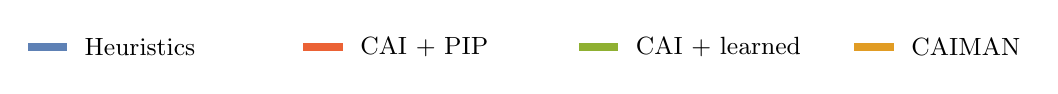
\begin{tikzpicture}
            % Legend entries
            \draw[draw=none, fill=heuristics] (0,0.1) rectangle (0.5,0.2); % rectangle
            \node[right] at (0.6,0.15) {\small{Heuristics}}; % text
            \draw[draw=none, fill=caiprior] (3.5,0.1) rectangle (4.0,0.2); % rectangle
            \node[right] at (4.1,0.15) {\small{CAI + PIP}}; % text
            \draw[draw=none, fill=cailearn] (7,0.1) rectangle (7.5,0.2); % rectangle
            \node[right] at (7.6,0.15) {\small{CAI + learned}}; % text
            \draw[draw=none, fill=caiman] (10.5,0.1) rectangle (11.0,0.2); % rectangle
            \node[right] at (11.1,0.15) {\small{CAIMAN}}; % text
        \end{tikzpicture}
    
    % Overall figure caption
    \caption{Policy success rate evaluated at every 100 training iterations for all methods and tasks. Results are averaged across 800 episodes and 3 seeds, shaded area represents standard deviation. }
    \label{fig:generalsuccess}
    \vspace{-0.5cm}
\end{figure*}

\section{Experiments}
\subsection{Task definitions}
We apply the proposed learning framework to three loco-manipulation pushing tasks of increasing difficulty, as illustrated in \Cref{fig:tasks} and detailed as follows:
\begin{itemize}
    \item \textbf{Single Object:} The single object task involves a singular cuboid object that the robot should manipulate to a target position. 
    \item \textbf{Single Wall:} The single wall task includes a fixed wall-like entity that blocks the direct path between the object and the target. The robot must navigate the object around the wall to push the object to the target position.
    \item \textbf{Multi-Wall:} The multi-wall task presents multiple fixed wall obstacles between the object and the target. The robot must learn to manipulate the object through these obstacles to reach the target position.
\end{itemize}

The fixed wall entities in the single-wall and multi-wall tasks create regions in the state space where the object’s kinematics become more complex, thereby affecting the degree of influence the robot can exert on the object in these states.
For all tasks, we train with a constant target position. 
A complete description of scene configurations is presented in \Cref{app:scene_configs}. 

\subsection{Experiment settings}
We train both high-level and low-level policies for Unitree Go2 (with a total mass of around 15 kilograms) in Issac Lab~\cite{mittal2023orbit} with parallelized environments.
In simulated tasks, the object has a length, width, and height of $0.5$ meters and a mass of $5.0$ kilograms, the wall in Single Wall has a length, width, and height of $(0.1, 1.0, 0.5)$ meters, and the walls in Multi-Wall have a length, width, and height of $(0.1, 1.25, 0.5)$ meters respectively. 
The training hyperparameters and additional training details can be found in~\Cref{app:hyperparams} and~\Cref{app:additional_training}.

We compare our approach against the following baselines:

\begin{itemize}
\item \textbf{Heuristics:} We train the high-level policy using a contact heuristic $r_{\text{heu}}$, formulated as $r_{\text{heu}} = \exp{-\norm{\boldsymbol{p}_r - \boldsymbol{p}_o}_2}$, in place of $r_{\text{CAI}}$. 
The contact heuristic encourages the robot to minimize the euclidean distance to the object and represents minimal effort task-specific reward engineering.
\item \textbf{CAI + PIP:} We train with $r_{\text{CAI}}$, where CAI is computed using only the physics-informed prior (PIP) dynamics model (\Cref{eq:PIP}), \ie without refining the dynamics model with a residual.

\item \textbf{CAI + learned:} We train with $r_{\text{CAI}}$ computed from dynamics that are fully learned, \ie without reliance on the physics informed prior. 
\end{itemize}
The second and third baselines serve as ablation studies of our proposed method to investigate the individual impacts of prior conditioning and online fine-tuning on overall training performance. 
For a detailed description of the reward functions and their coefficients, see \Cref{app:reward}. 

\subsection{Simulation results}
We evaluate the learning performance of each method by calculating the success rate of policies for each task. 
A task is defined to be successfully completed if the distance between the object and the target is under a certain threshold $\epsilon_s$ at the end of the episode, and the success rate is thus calculated as the number of environments with successful task completion out of the total number of environments used for evaluation. 
For every task, each method is evaluated on 800 episodes averaged across 3 different seeds.

The results are presented in \Cref{fig:generalsuccess} and \Cref{tab:success_rate}.

\begin{table}[!t]
\vspace{0.2cm}
\centering

\begin{tabular}{@{\extracolsep{\fill}}lccc}
\toprule
\multirow{2}{*}{\textbf{Method}} & \multicolumn{3}{c}{\textbf{Task}} \\ 
\cmidrule(lr){2-4}
& Single Object & Single Wall & Multi-Wall \\ 
\midrule
Heuristics & 0.93 $\pm$ 0.02
           & 0.0 $\pm$ 0.0
           & 0.0 $\pm$ 0.0 \\
CAI + PIP  & 0.80 $\pm$ 0.04
                    & 0.0 $\pm$ 0.0
                    & 0.0 $\pm$ 0.0\\
CAI + learned & 0.73 $\pm$ 0.06
                       & 0.21 $\pm$ 0.19
                       & 0.16 $\pm$ 0.22\\
CAIMAN  & \textbf{0.98} $\pm$ 0.01
        & \textbf{0.94} $\pm$ 0.04
        & \textbf{0.96} $\pm$ 0.02\\

\bottomrule
\end{tabular}
\caption{Final success rates under all methods for each task. Results are averaged across 800 episodes and 3 independent seeds.
}
\label{tab:success_rate}
\vspace{-0.5cm}
\end{table}

\begin{figure}[t!]
    \centering
        \begin{minipage}{0.2\textwidth}
            \centering
            \includegraphics[width=\linewidth]{original_figures/results/trajectory_heuristic.png}
        \end{minipage}%
        \hspace{0.005\textwidth}
        \begin{minipage}{0.2\textwidth}
            \centering
            \includegraphics[width=\linewidth]{original_figures/results/trajectory_pip.png}
        \end{minipage}%
        \vspace{0.01\textwidth}  % Vertical space between rows
        
        \begin{minipage}{0.2\textwidth}
            \centering
            \includegraphics[width=\linewidth]{original_figures/results/trajectory_learned.png}
        \end{minipage}%
        \hspace{0.005\textwidth}
        \begin{minipage}{0.2\textwidth}
            \centering
            \includegraphics[width=\linewidth]{original_figures/results/trajectory_caiman.png}
        \end{minipage}%
        \vspace{0.005\textwidth}  % Vertical space between rows
    \caption{HL policy trajectories under different methods for the sparse reward multi-wall task. Heuristics (\textit{top left}), CAI+PIP (\textit{top right}), CAI+learned (\textit{bottom left}), CAIMAN (\textit{bottom right}). }
    \label{fig:top_trajectories}
    % \vspace{-0.5cm}
\end{figure}

\begin{figure}[t!]
    \centering
    \includegraphics[width=0.75\linewidth]{original_figures/task_transfer_singlewall.png}
    \caption{Single wall task with target positions randomly sampled within an area in front of the wall. }
    \label{fig:random_target_task}
    % \vspace{-0.5cm}
\end{figure}

\begin{figure}[t!]
    \centering
    \includegraphics[width=0.8\linewidth]{original_figures/results/transfer_singlewall.pdf}
    \caption{Learning the single wall random target task using learning from scratch and learning with models transferred from the fixed target task. }
    \label{fig:transfer}
    \vspace{-0.5cm}
\end{figure}

With a sparse task reward, task-relevant skill learning is primarily driven through exploration. 
All methods achieve some degree of success in the single-object task, with CAIMAN and heuristic-based approaches outperforming CAI + PIP and CAI + learned.
CAI + learned exhibits the poorest performance due to the time and data required to learn an accurate dynamics model, whereas CAI + PIP performs more comparably to CAIMAN and heuristic methods.
This suggests that the naive PIP dynamics model is sufficient for simple tasks with relatively simple interactions.

For the more complex single wall and multi-wall tasks, only CAIMAN achieves significant success. 
This suggests that our method is uniquely capable of facilitating efficient task-solving exploration in the presence of obstacles, validating its effectiveness in cluttered environments in the absence of dense extrinsic task reward signals.
Furthermore, the failure of CAI + PIP and CAI + learned to provide satisfactory dynamics for effective exploration in sparse-wall tasks highlights the necessity of combining prior dynamics with a learned residual model in complex environments.

\Cref{fig:top_trajectories} illustrates example trajectories of policies trained using different methods for the multi-wall task.


\subsection{Leveraging pretrained dynamics for new tasks}
Since our framework entails learning the environment dynamics, we can leverage the learned dynamics model from one task for another, provided that the underlying dynamics remain unchanged.
We hypothesize that utilizing a pretrained dynamics will result in more accurate CAI measures at early stages of training, hence improving the quality of the exploration signal and leading to significant gains in sample efficiency.
We demonstrate this concept on the single wall task with random target positions sampled uniformly within a predefined area, as illustrated in~\Cref{fig:random_target_task}.
This serves as a generalization of the single wall task with a fixed target position from the previous section. 
The detailed scene configuration is provided in~\Cref{app:scene_configs}.

We compare the performance of the CAIMAN framework with dynamics trained from scratch to a CAIMAN variant that reuses pretrained dynamics.

For the variant, we reuse the same PIP model and a previously learned residual, and continue fine-tuning the residual model with new interactions from the generalized task.
As shown in \Cref{fig:transfer}, reusing the learned dynamics from the previous task significantly accelerates learning under the sparse task reward. 
The pretrained dynamics model provides better exploration through CAI, enabling the robot to exhibit meaningful interaction behaviors early in the training process, leading to significant gains in sample efficiency, thus confirming our hypothesis.

\subsection{Hardware deployment}
\begin{figure} %[t]
    \centering
    \begin{subfigure}[b]{\linewidth}
    \includegraphics[width=\linewidth]{original_figures/hw1.png}
    \end{subfigure}
    \par\medskip
    \begin{subfigure}[b]{\linewidth}
    \includegraphics[width=\linewidth]{original_figures/hw2.png}
    \end{subfigure}

    \caption{Snapshots from the hardware deployment for the single object and single wall tasks. The mass of the box is 5.5 kilograms with a dimension of $(0.55, 0.55, 0.5)$ meters. } 
    \label{fig:Hardware}
    \vspace{-0.5cm}
\end{figure}

We validated our trained policy on the Unitree Go2, as shown in \Cref{fig:Hardware}.
Since hardware execution demands higher-quality motions, we retrained the low-level policy to improve robustness in velocity tracking.
Additionally, to account for physical discrepancies between simulation and our real-world setup, we applied domain randomization on object mass and friction during high-level policy training. 
For additional details, refer to \Cref{app:dr_hw}.
All entities in the environment were tracked using a motion capture system, providing accurate pose observations for both high- and low-level policies.
The trained policies were deployed directly onto the robot without any additional fine-tuning, demonstrating the strong sim-to-real transfer capability of the high-level policy trained with \method.

\section{Conclusion}
We present \method, a novel learning framework for training loco-manipulation skills in legged robots using only sparse extrinsic task rewards.
Leveraging an intrinsic motivation exploration bonus that encourages the agent to gain causal influence over other entities in the environment, \method eliminates the need for tedious, hand-engineered task-specific rewards, even in complex scenarios.
We demonstrate the effectiveness of our method by using a quadruped robot to push a large and heavy object to a target location.
Through extensive simulation experiments, we show that \method achieves superior sample efficiency compared to baseline methods, particularly in environments with obstacles.
Additionally, we demonstrate the effectiveness of combining a physics-informed prior with a learned residual model to improve the accuracy of the learned dynamics model.
Furthermore, we illustrate that the learned dynamics model from our framework can be leveraged to enhance learning efficiency in new tasks.
Finally, we successfully validate our approach on hardware without any additional fine-tuning, demonstrating its seamless transferability to real-world applications.

\section{Limitations}
Although CAI-based exploration provides meaningful guidance for robot-object interaction, it inevitably relies heavily on an accurate dynamics model.
Currently, \method trains the high-level policy alongside the dynamics residual, which may lead to undesired exploratory behaviors in the early stages of training when the dynamics model is still inaccurate.
Leveraging a pretrained world model could help mitigate this issue.
When transferring the learned dynamics, \method operates under the assumption that the environment remains unchanged.
If the environment undergoes changes, a potential approach to address this challenge is fine-tuning the learned dynamics model in the new environment.
Additionally, \method leverages CAI for exploring single-object interaction only.
A potential direction for future work is extending \method to enable exploration of multi-object interactions.

\section*{Acknowledgments}
We thank Dongho Kang, Taerim Yoon, Zijun Hui, Flavio De Vincenti and Hélène Stefanelli for developing the hardware testing framework.

\bibliographystyle{unsrtnat}
\bibliography{references}

\newpage
\begin{appendices}
\counterwithin{figure}{section}
\counterwithin{table}{section}

\onecolumn

\section{Detailed Observation Space}
\label{app:obs}
Below we list the observation space for low-level, high-level policies and the high-level state for calculating CAI. 

\begin{table}[!ht]
    \centering
    \renewcommand{\arraystretch}{1.1}
    \begin{tabular}{|c|c|}
        \hline
        \multicolumn{2}{|c|}{\textbf{Low-level observation} $\boldsymbol{o}_l$} \\ \hline
        $_{\mathcal{B}}\boldsymbol{v}_r\in\mathbb{R}^3$ & robot linear velocity in base frame $\mathcal{B}$ \\ \hline
        $_{\mathcal{B}}\boldsymbol{\omega}_r\in\mathbb{R}^3$   & robot angular velocity in base frame $\mathcal{B}$  \\ \hline
        $\boldsymbol{q}_j\in\mathbb{R}^{12}$   & Joint positions   \\ \hline
        $\Dot{\boldsymbol{q}}_j\in\mathbb{R}^{12}$   & Joint velocities   \\ \hline
        $_{\mathcal{B}}\boldsymbol{g}\in\mathbb{R}^3$   & Projected gravity in base frame $\mathcal{B}$ \\ \hline
        $\boldsymbol{v}_{r,des}=(v^x_{r,des}, v^y_{r,des}, \omega^z_{r,des})\in\mathbb{R}^3$   & Desired velocity command \\ \hline
        $\boldsymbol{a}_{l,prev}\in\mathbb{R}^{12}$& Previous action  \\ \hline\hline
        
        \multicolumn{2}{|c|}{\textbf{High-level observation} $\boldsymbol{o}_h$ (in world frame $\mathcal{W})$} \\ \hline
        $\boldsymbol{v}_r\in\mathbb{R}^3$   & Robot linear velocity \\ \hline
        $\boldsymbol{\omega}_r\in\mathbb{R}^3$   & Robot angular velocity \\ \hline
        $\boldsymbol{\xi}_r = (x_r, y_r, \psi_r)\in\mathbb{R}^3$   & Robot pose\\ \hline
        $\boldsymbol{\xi}_o = (x_o, y_o, \psi_o)\in\mathbb{R}^3$   & Object pose\\ \hline
        $\boldsymbol{p}_{t} = (x_t, y_t)\in\mathbb{R}^2$   & Target position\\ \hline
        $\boldsymbol{a}_{h, prev}\in\mathbb{R}^3$   & Previous action\\ \hline
        \multicolumn{2}{|l|}{\textit{additional:}} \\ \hline
        $(x_w, y_w, \psi_w)\in\mathbb{R}^3$   & Wall pose (for each wall)\\ \hline\hline
        
        \multicolumn{2}{|c|}{\textbf{high-level state for CAI} $\boldsymbol{s}_h$ (in world frame $\mathcal{W}$)} \\ \hline
        $\boldsymbol{\xi}_r = (x_r, y_r, \psi_r)\in\mathbb{R}^3$   & Robot pose\\ \hline
        $\boldsymbol{\xi}_o = (x_o, y_o, \psi_o)\in\mathbb{R}^3$   & Object pose\\ \hline
        $\boldsymbol{v}_r = (v_r^x, v_r^y, \omega_r^z)\in\mathbb{R}^3$   & Robot velocity \\ \hline
        $\boldsymbol{v}_o = (v_o^x, v_o^y, v_o^z)\in\mathbb{R}^3$   & Object velocity \\ \hline

    \end{tabular}
    \caption{Detailed observation space for each module.}
    \label{tab:obs}
\end{table}


\section{Scene Configurations}
\label{app:scene_configs}
The detailed initial pose for each entity and target position are shown in \Cref{tab:initial_configs}.
\begin{table}[!ht]
    \centering
    \renewcommand{\arraystretch}{1.1}
    \begin{tabular}{|c|c|c|c|c|}
    \hline
       \textbf{Task}  &  Single Object & Single Wall & Multi-Wall & Single Wall (Transfer) \\ \hline
    \textbf{Robot} & (0.0, 0.0, $\mathcal{U}(-\pi, \pi]$) & (0.0, 0.0, $\mathcal{U}(-\pi, \pi]$) & (0.0, 0.0, $\mathcal{U}(-\pi, \pi]$) & (0.0, 0.0, $\mathcal{U}(-\pi, \pi]$)\\ \hline
    \textbf{Object} & (1.0, 0.0, 0.0) & (1.0, 0.0, 0.0) & (1.0, 0.0, 0.0) & (1.0, 0.0, 0.0)\\ \hline
    \textbf{Target} & (3.0, 0.0) & (3.5, 0.0) & (4.0, 0.0) & ($\mathcal{U}[3.0, 4.0]$, $\mathcal{U}[-1.0, 1.0]$)\\ \hline
    \textbf{Wall 1} & - & (2.0, 0.0, 0.0) & (2.0, 0.0, 0.0) & (2.0, 0.0, 0.0) \\ \hline
    \textbf{Wall 2} & - & - & (3.25, 1.25, 0.0) & - \\ \hline
    \textbf{Wall 3} & - & - & (3.25, -1.25, 0.0) & - \\ \hline
    \end{tabular}
    \caption{We list the scene configurations, where the initial pose $(x, y, \psi)$ for every existing entity and the target position $(x, y)$ for each task (Single Object, Single Wall, Multi-Wall) is shown. 
    }
    \label{tab:initial_configs}
\end{table}

\newpage

\section{Rewards and Coefficients}
\label{app:reward}
We list the reward functions and corresponding reward parameters for all tasks and training methods in \Cref{tab:rewards}. 
\begin{table}[!h]
    \centering
    \setlength{\tabcolsep}{4pt}
    \renewcommand{\arraystretch}{1.2}
    \begin{tabular}{|c|c|}
         \hline
         \multicolumn{2}{|c|}{\textbf{Reward functions}} \\ \hline
         CAI &$r = w_1r_{\text{task}} + w_2r_{\text{CAI}} + w_3r_{\text{reg}} $ \\
         \hline
         heuristic & $r = w_1r_{\text{task}} + w_4r_{\text{heu}} + w_3r_{\text{reg}} $ \\
         \hline
         $r_{\text{CAI}}$ weight & \Cref{eq:cai_weight} \\
         \hline
    \end{tabular}
    
    \vspace{6pt}
    \begin{tabular}{|c|c|c|c|c|c|c|}
        \hline
         \multicolumn{7}{|c|}{\textbf{Reward coefficients}} \\ \hline
         \textbf{Task} & \textbf{$w_1$} & \textbf{$w_3$} & \textbf{$w_4$} & \textbf{$w_{2, b}$} & \textbf{$\alpha_1$} & \textbf{$\alpha_2$}\\ \hline
         Single object & 15 & -5e-3 & 0.01 & 40 & 12e-5 & 1.5e-6 \\ \hline
         Single wall & 40 & -5e-3 & 0.01 & 40 & 12e-5 & 1.5e-6 \\ \hline
         Multi-wall & 40 & -5e-3 & 0.01 & 40 & 12e-5 & 1.5e-6 \\ \hline
    \end{tabular}
    \caption{Simulation training reward parameters. All CAI methods (CAI + PIP, CAI + Learned, \method) use the CAI reward function, while the heuristic reward function is only applied to the heuristics method.}
    \label{tab:rewards}
\end{table}

\section{Hyperparameters}
We list all the hyperparameters used for training the high-level loco-manipulation policy and dynamics residual model in \Cref{tab:hyperparams}.
\label{app:hyperparams}
\begin{table}[h]
\centering
   \vspace{6pt}
    \begin{tabular}{|c|c|}
         \hline

        \multicolumn{2}{|c|}{\textbf{Environment hyperparameters}} \\ \hline
        number of environments & 4096 \\ \hline
        $v_{r,des}^{x}$ (m/s)   & $[-1.0, 1.0]$ \\ \hline 
        $v_{r,des}^{y}$ (m/s)   & $[-1.0, 1.0]$ \\ \hline  
        $\omega_{r,des}^{z}$ (rad/s) & $[-1.0, 1.0]$\\ \hline  
        $\delta{v}_r^{x}$ (m/s)   & $0.3$\\ \hline  $\delta{v}_r^{y}$ (m/s)   & $0.3$\\ \hline  $\delta{\omega}_r^{z}$ (rad/s) & $0.4$\\ \hline  
        threshold for PIP dynamics $\epsilon_p$ (m) & $0.7$\\ \hline
        threshold for sparse task reward $\epsilon$ (m) & $0.1$\\ \hline
        success rate threshold $\epsilon_s$ (m)& $0.15$ \\ \hline
        high-level policy frequency (Hz) & $5$ \\\hline
        low-level policy frequency (Hz) & $50$ \\\hline
        number of sampled action in CAI $K$ & 64 \\ \hline\hline


        \multicolumn{2}{|c|}{\textbf{PPO hyperparameters}} \\ \hline
        policy network & $[512, 256, 128]$ \\ \hline
        policy activation function & ELU \\ \hline
        policy initial standard deviation & $1.0$ \\ \hline
        value network & $[512, 256, 128]$ \\ \hline
        value activation function & ELU \\ \hline
        number of mini-batches & $4$ \\ \hline
        number of epochs per iteration & $5$ \\ \hline
        clip threshold & $0.2$ \\ \hline
        learning rate schedule & adaptive \\ \hline
        desired KL divergence & $0.01$ \\ \hline
        value function loss coefficient & $1.0$ \\ \hline
        entropy coefficient & $0.005$ \\ \hline
        max gradient norm & $1.0$ \\ \hline
        $\gamma$ & $0.99$ \\ \hline
        $\lambda$ & $0.95$ \\ \hline \hline

        \multicolumn{2}{|c|}{\textbf{Dynamics hyperparameters}} \\ \hline
        fixed variance $\sigma$ & $1.0$ \\ \hline
        residual model & $[256, 128]$ \\ \hline
        batch size & $4096$ \\ \hline
        number of epochs per iteration & $8$ \\ \hline
        learning rate & $0.0001$ \\ \hline
        buffer size & $10000000$ \\ \hline
        
    \end{tabular}
    \caption{High-level policy and dynamics residual training hyperparameters.}
    \label{tab:hyperparams}
\end{table}

\section{Additional training details}
\label{app:additional_training}
The low-level policy operates with a control interval of 0.02 seconds, while the high-level policy has a control interval of 0.2 seconds. 
For every iteration through the high-level control loop, we step the environment by 0.2 seconds, compute the rewards and terminations, collect transitions for the high-level and dynamics policies, and calculate and add the CAI exploration bonus to the rewards buffer.
We trained 1500 iterations for the single object and single wall tasks and 2000 iterations for the multi-wall task, where each iteration consists of 10 high-level control steps. 
All tasks have an episode length of 20 seconds.

In addition to CAI, we also generate meaningful exploration through colored noise during policy rolling out~\cite{eberhard2023pink, hollenstein2024colored}. 
By sampling from time-correlated actions, we reduce the possibility of meaningless back-and-forth behavior that could result from commonly used white noise. 
We select a correlation strength parameterized as $\beta = 0.5$, corresponding to a colored noise between white and pink. 


\section{Domain randomization for hardware deployment}
\label{app:dr_hw}
\Cref{tab:HWrandomization} presents the environment parameters that were randomized in simulation during training policies for hardware deployment.
\begin{table}[!ht]
    \centering

    \begin{tabular}{|c|c|}
         \hline
         \textbf{Parameter} & \textbf{Range} \\
         \hline
         Object mass $(kg)$ &  $\mathcal{U}[3.5, 7.5]$ \\
         Object friction coefficient & $\mathcal{U}[0.5, 1.5]$ \\
         Initial robot position $(m)$ & x: $\mathcal{U}[-0.1, 0.1]$, y: $\mathcal{U}[-0.1, 0.1]$ \\
         Initial object position $(m)$ & x: $\mathcal{U}[0.9, 1.1]$, y: $\mathcal{U}[-0.1, 0.1]$ \\
         \hline
    \end{tabular}
    \caption{Randomized parameters in simulation for training HL policies for hardware.}
    \label{tab:HWrandomization}
\end{table}


\section{Dense task reward}
Though we primarily focused on a sparse task reward, we also trained all tasks in simulation under a dense task reward for all methods. The dense task reward, defined as $r_{\text{task}}^{dense} = \exp{-\norm{\boldsymbol{p}_{o} - \boldsymbol{p}_{t}}_2}$, awards an amount inversely proportional to the euclidean distance between the object and the target. 

The final success rates for all methods after training under a dense task reward is summarized in \Cref{tab:dense_success_rate}, and task performance during training is shown in \Cref{fig:dense_plots}. 
For learning the single object task with dense rewards, all methods demonstrate similar learning speeds and success rates, which indicates that within simpler, less cluttered environments, a dense reward scheme sufficiently guides task learning.
However, for the dense reward single wall and multi-wall tasks, all CAI-imbued learning methods (CAIMAN, CAI + PIP, CAI + learned) exhibit better sample efficiency over the heuristics method, indicating that learning the actions necessary for obstacle navigation is facilitated through CAI exploration. 
CAIMAN and CAI + PIP achieve the fastest convergence and the highest success rates, while CAI + learned is slightly less sample efficient. 
This can be attributed to the fact that learning dynamics from scratch initially produces erroneous predictions, which results in inaccurately high CAI scores and diverts the robot from acquiring task specific skills. 
In contrast, with the PIP only dynamics model, the resulting exploration behavior is less adversely impacted when skill learning is heavily guided by dense rewards.

\begin{table}[!ht]
\centering

\begin{tabular}{@{\extracolsep{\fill}}lccc}
\toprule
\multirow{2}{*}{\textbf{Method}} & \multicolumn{3}{c}{\textbf{Task}} \\ 
\cmidrule(lr){2-4}
& Single Object & Single Wall & Multi-Wall \\
\midrule
Heuristics & 0.957 $\pm$ 0.004
           & 0.543 $\pm$ 0.471 
           & 0.799 $\pm$ 0.341 \\
CAI + PIP & 0.942 $\pm$ 0.005
                    & 0.979 $\pm$ 0.008
                    & \textbf{0.955} $\pm$ 0.008
                    \\
CAI + learned & 0.908 $\pm$ 0.033 
                       & 0.935 $\pm$ 0.011 
                       & 0.895 $\pm$ 0.042
                       \\
CAIMAN & \textbf{0.961} $\pm$ 0.003
                                    & \textbf{0.990} $\pm$ 0.004 
                                    & 0.954 $\pm$ 0.028
                                    \\

\bottomrule
\end{tabular}
\caption{Final policy success rates evaluated after training completion under a dense task reward.}
\label{tab:dense_success_rate}
\end{table}

\begin{figure*}[ht]
    \centering
        %\centering
         \begin{minipage}{0.33\textwidth}
            \centering
            \includegraphics[width=\linewidth]{original_figures/results/dense_singleobject.pdf}
        \end{minipage}%
        \begin{minipage}{0.33\textwidth}
            \centering
            \includegraphics[width=\linewidth]{original_figures/results/dense_singlewall.pdf}
        \end{minipage}%
        \begin{minipage}{0.33\textwidth}
            \centering
            \includegraphics[width=\linewidth]{original_figures/results/dense_multiwall.pdf}
        \end{minipage}

        \vspace{.5em}
        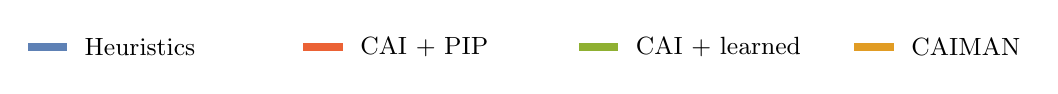
\begin{tikzpicture}
            \draw[draw=none, fill=heuristics] (0,0.1) rectangle (0.5,0.2); % rectangle
            \node[right] at (0.6,0.15) {\small{Heuristics}}; % text
            \draw[draw=none, fill=caiprior] (3.5,0.1) rectangle (4.0,0.2); % rectangle
            \node[right] at (4.1,0.15) {\small{CAI + PIP}}; % text
            \draw[draw=none, fill=cailearn] (7,0.1) rectangle (7.5,0.2); % rectangle
            \node[right] at (7.6,0.15) {\small{CAI + learned}}; % text
            \draw[draw=none, fill=caiman] (10.5,0.1) rectangle (11.0,0.2); % rectangle
            \node[right] at (11.1,0.15) {\small{CAIMAN}}; % text
        \end{tikzpicture}
    
    % Overall figure caption
    \caption{Policy success rate during training under a dense task reward for all methods. All experiments utilize a minimum of 2 seeds.}
    
    % Label for referencing the figure
    \label{fig:dense_plots}
\end{figure*}
    
\end{appendices}
\end{document}


